\documentclass[12pt,a4paper]{article}

\usepackage{german}      % Deutsche TeX-Eigenheiten
\usepackage{sectsty}
\usepackage{xcolor}
\usepackage{makeidx}
\makeindex            % damit eine Indexdatei angelegt wird

\usepackage{graphicx}

\usepackage{amsmath}  % allgemeine Mathe-Erweiterungen
\usepackage{amssymb}  % Symbole und Schriftarten
\usepackage{amsthm}   % erweiterte Theorem-Umgebungen

\usepackage{mathrsfs}  % gibt den Befehl "\mathscr{}" f�r sch�ne

\begin{document}
Mathematik für Informatiker II - Arthur Kunze
\section*{Aufgabe 11}
$\int_{1}^{e}\frac{ln(x)}{x\cdot \sqrt{1+(ln(x))^2}}dx \qquad  u=ln(x)=g(x) \qquad g'(x)=\frac{1}{x} \rightarrow dx=\frac{du}{\frac{1}{x}} \quad du=\frac{1}{x}dx$\\
\\
$\int_{1}^{e}\frac{u}{\sqrt{1+u^2}}du = \sqrt{1+u^2} = \sqrt{1+(ln(x))^2}+C$\\
\\
$\int_{1}^{e}\frac{ln(x)}{x\cdot \sqrt{1+(ln(x))^2}}dx = \left[\sqrt{1+(ln(x))^2}\right]_1^e = \sqrt{1+(ln(e))^2}-\sqrt{1+(ln(1))^2}$\\
\\
$=\sqrt{1+(1)^2}-\sqrt{1+(0)^2}=\sqrt{2}-\sqrt{1} \approx 0,4132$\\
\\
\section*{Aufgabe 12}
$f(x)=x^2, \quad g(x)=2x, \quad [0,4]$\\
\\
Der Schnittpunkt bei $x=2$ teilt die Fläche $A$ in $A_1+A_2$\\
\\
$A_1=\int_0^2(g(x)-f(x))dx \qquad A_2=\int_2^4(f(x)-g(x))dx$\\
\\
$A_1=\int_0^2(2x-x^2)dx=\int_0^2-x^2+2x \hspace{0.2cm} dx$\\
\\
$=-\frac{1}{3}x^3+x^2+C = \left[-\frac{1}{3}x^3+x^2\right]_0^2$\\
\\
$=(-\frac{1}{3}2^3+2^2)-(-\frac{1}{3}0^3+0^2)=(-\frac{8}{3}+4)-(0+0)$\\
\\
$=-\frac{8}{3}+\frac{12}{3}=\frac{4}{3}$\\
\\
$A_2=\int_2^4(x^2-2)dx = \frac{1}{3}x^3-x^2$\\
\\
$=\left[\frac{1}{3}x^3-x^2\right]_2^4=(\frac{1}{3}4^3-4^2)-(\frac{1}{3}2^3-2^2)$\\
\\
$=(\frac{64}{3}-16)-(\frac{8}{3}-4)=(\frac{64}{3}-\frac{48}{3})-(\frac{8}{3}-\frac{12}{3})$\\
\\
$=\frac{16}{3}+\frac{4}{3}=\frac{20}{3}$\\
\\
$\rightarrow A=A_1+A_2=\frac{4}{3}+\frac{20}{3}=\frac{24}{3}=8$\\
\\
\section*{Aufgabe 13}
$\int_0^1xln(x)dx$\quad Unstetigkeitsstelle $=0$; stetig in $(0,1]$\\
\\
Unbeschränkt für $x\rightarrow 0$
\\
Stammfunktion: $\frac{1}{2}x^2ln(x)-\frac{1}{4}x^2+C=x^2(\frac{1}{2}ln(x)-\frac{1}{4}+C)$\\
\\
Bestimmtes Integral: $\int_\alpha^1xln(x)dx = \lim \limits_{\alpha\rightarrow 0; \alpha > 0}\left[x^2(\frac{1}{2}ln(x)-\frac{1}{4}\right]_\alpha^1$\\
\\
$=1^2(\frac{1}{2}ln(1)-\frac{1}{4})-\lim \limits_{\alpha\rightarrow 0; \alpha > 0}\alpha^2(\frac{1}{2}ln(\alpha)-\frac{1}{4})$\\
\\
$=\underbrace{(\frac{1}{2}ln(1)-\frac{1}{4})}_{=\frac{1}{2}\cdot 0-\frac{1}{4}=-\frac{1}{4}}-(\lim \limits_{\alpha\rightarrow 0; \alpha > 0}\frac{1}{2}\underbrace{\underbrace{\alpha^2}_{\rightarrow 0}\underbrace{ln(\alpha)}_{\rightarrow -\infty}}_{``0\cdot -\infty``}-\alpha^2\frac{1}{4})$
\\
Zum L'Hospital:\\
$\lim \limits_{\alpha\rightarrow 0; \alpha > 0}\alpha^2ln(\alpha)\underbrace{=}_{``0\cdot -\infty``}\lim \limits_{\alpha\rightarrow 0; \alpha > 0}\frac{ln(\alpha)}{\frac{1}{\alpha^2}}$\\
\\
$\underbrace{=}_{``\frac{-\infty}{\infty}``}\lim \limits_{\alpha\rightarrow 0; \alpha > 0}\frac{\frac{1}{\alpha}}{-\frac{2}{\alpha^3}}=\lim \limits_{\alpha\rightarrow 0; \alpha > 0}-\frac{\alpha^3}{2\alpha}\rightarrow 0$\
\\
Der zweite Term geht gegen $0$ und somit ist das Ergebnis $-\frac{1}{4}$\\
Dadruch ist das uneigentliche Integral \textbf{konvegent}.\\
\\
\newpage
\section*{Aufgabe 14}
$\int_\frac{1}{2}^\infty \frac{1}{\sqrt{x(1+x^2)}}dx = \int_\frac{1}{2}^\infty \frac{1}{\sqrt{x+x^3}}dx$\\
\\
Für $\int_1^\infty$:\\
$|f(x)|=\frac{1}{\sqrt{x+x^3}} = \frac{1}{(x+x^3)^\frac{1}{2}}\leq \frac{1}{(x^3)^\frac{1}{2}}=\frac{1}{x^{3\cdot \frac{1}{2}}}= \frac{1}{x^\frac{3}{2}}$\\
\\
Da $\frac{3}{2} > 1$ \textbf{konvergiert} dieser Abschnitt (Majorantenkriterium).\\
\\
Für $\int_\frac{1}{2}^1$:\\
Da man die Grenzen ($\frac{1}{2}$ und $1$) und den Bereich im Intervall \\
(zwischen $\frac{1}{2}$ und $1$) problemlos einsetzten kann und \\ 
es keine Unstetigkeitsstellen gibt, ist dieser Abschnitt \textbf{konvergent}\\
Damit folgt, dass das ganze uneigentliche Integral \textbf{konvergent} ist.\\
\\
\section*{Aufgabe 15}
$f(x)=\begin{cases}
               1,\quad -\pi < x \leq 0\\
               x,\quad 0 < x \leq \pi\\
        \end{cases}$\\
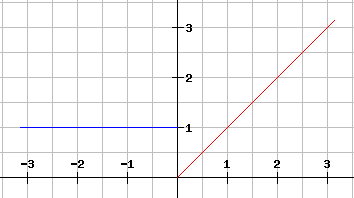
\includegraphics[width=0.3\textwidth]{skizze.png}
\\
$a_0=\frac{1}{2\pi}\cdot \int_{-\pi}^\pi f(x)dx = \frac{1}{2\pi}(\int_{-\pi}^0 1dx+\int_0^\pi xdx)$\\
\\
$=\frac{1}{2\pi}(\left[x\right]_{-\pi}^0+\left[\frac{x^2}{2}\right]_{0}^\pi)=\frac{1}{2\pi}((0-(-\pi))+(\frac{\pi^2}{2}-\frac{0^2}{2}))=\frac{1}{2\pi}(\pi+\frac{\pi^2}{2})$\\
\end{document} 